\documentclass[11pt]
{article}
\usepackage{graphicx}
\usepackage{subcaption}
\usepackage{float}
\usepackage{hyperref}
\usepackage[bottom]{footmisc}
\usepackage{babel}[English]
\usepackage{apacite}

\title{DL LAB 2: An application with RNN}
\author{Senne Deproost and Diego Saby}
\date{November 2019}


\begin{document}
\maketitle
\section{Introduction}
In the field of machine learning we try create computational models to find solutions for a wide set of tasks. One of the more popular problems to solve are the classification of instances and function approximation with regression. Solutions like \textit{Support Vector Machines} and \textit{Decision Trees} have already proven their worth in the past. Techniques from the deep learning (DL) sub-field of machine learning have shown their usability when tackling on data with high dimen\-sionality. Deep learning's ability to scale better with these kinds of data makes it useful in many application domains like machine control and decision support systems. Variations in the model's architecture could insure better performance on a domain specific task.\\

One DL architecture we'll focus on in this lab report is the \textit{Recurrent Neural Network} architecture. Whereas classical \textit{Feedforward Neural Network} (FNN) only allows the passage of activation through the neuron layers, a RNN network will remember the neuron activations from a previous step in time. This is implemented with the inclusion of memory nodes that will hold on to previous encountered activation values. An advantage of this kind of networks is the usage of \textit{Temporal Sequences}, allowing the model to train on data like text sentences, music recordings and streams of data.\\

Automated content creation using DL models has known a significant rise in popularity over the past years. With \textit{Generative Adverserial Networks} (GAN's), we can use two competing networks to train a generator for images \cite{Goodfellow2014}. In this architecture, one network, the has to mimic given image data input distribution and another adversarial network that has to estimate the loss of the predicted regression with given training data. This prediction can then be used to optimize the generative network. Other types of models like \textit{transformers}, recently used in OpenAI's GPT-2 model \cite{Radford}, can generate human-like text paragraphs with the potential of passing the famous Turing test. With a rise in the exploration of the generative content field, researches already used RNN based models to generate content like images \cite{Gregor}, voice synthesis \cite{Oord2016,VanDenOord2016} and music \cite{Oord2016}.\\

Music generation can be seen as a series of notes. We can try to predict the next note given the previous series of notes.
For this kind of problem RNNs are useful.

\subsection{Problem}
In this report, we will focus on three types of models in the task of creating music from MIDI files. The data will consists of fragments of Chopin's Nocturne music composition in the MIDI file format with 30 available notes available on the tone ladder. The music consists of only one music instrument: the piano.

Apart from regular RNNs, we will experiment on \textit{Long Short-Term Memory} (LSTM)\cite{Hochreiter:1997:LSM:1246443.1246450} and \textit{Gated Recurrent Unit } (GRU) models \cite{Cho}.

\subsection{LSTM}
An LSTM is a form of RNN which solves the problem of the large decay in loss function gradient over long periods of time. Specialized memory cells are used to recall on several past activations for longer periods of time. In addition, the network contains gates to control the information flow to and from memory and when it can be returned to its initial status.

\subsection{GRU}
GRU are similar in construction to LSTM that they have gates to control the specialized memory cells. However, these models are simplified containing less gates and dont make the distinction between memory cells and normal ones \cite{Chung}.

\begin{figure}[H]
	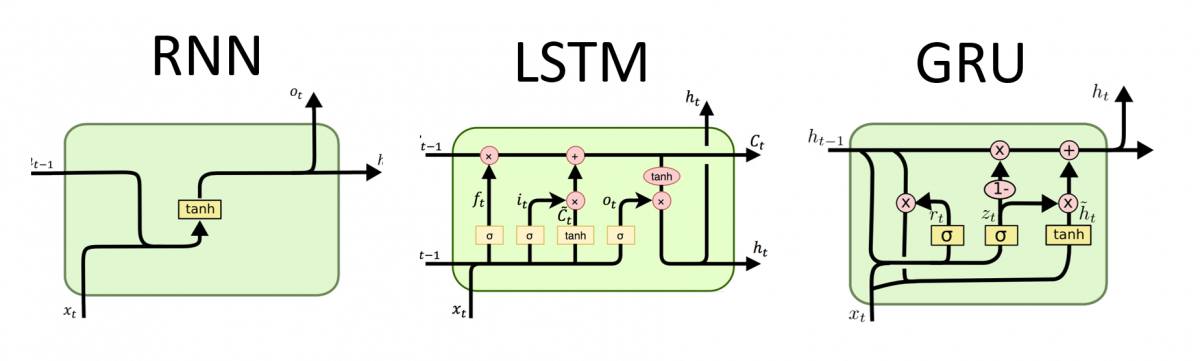
\includegraphics[width=\linewidth]{comp.png}
	\caption{An overview of the three kinds of models used in the experiments. Left we have a simple RNN node containing a simple $tanh$ activation function. In the middle the internal gates of the LSTM node are shown. The right contains the simplified layout of a GRU network node.}
	\label{fig:fig1}
\end{figure}


%\begin{itemize}
%	\item talk about RNN and LSTM
%	\item Talk about how RNN is useful for music
%	\item Introduce our project -> RNN on Chopin Nocturnes
%	\item Something else?...
%\end{itemize}


\section{Preprocess the data}
One of the first questions we were opposed to was how to encode music in order to train the Neural Network. Our source files are midi files. They are an useful way to encode the music where we can extract the notes and their duration from the file.\\
To simplify the problem we decided to abstract the notes duration and just use the notes pitch. \\

\subsection{Enumerating the notes}
Our first attempt was done inspired by some code found on the internet to produce video games music\footnote{https://github.com/Skuldur/Classical-Piano-Composer}.\\
To extract the notes the notes from midi file we used a library called \textit{Music21}. It provided us with the notes names or chord names that were played. From there we have a sequence of notes names. Then we just assign the notes a number from 1 to the length of the vocabulary (notes and chord names).
For the prediction we used a vector of all the notes and a with 1 for the next note that follows the sequence and 0 for the others.\\
After several experiments using a as the last layer a Fully connected NN with a \textit{softmax} activation function and taking the note with the biggest probability to be the next one as the prediction of the next note, the results were disappointing
 No matter what was the input it always yielded the same note. After changing the RNN architecture, the learning rate, the optimization function, it changed the note that was predicted, but always was a sequence of the same  note.

\subsection{Notes as Integers}
Our second approach was to translate directly a note pitch into an integer. 
The lower the pitch the bigger the integer.
This could be done thanks to another library called \textit{mido}, and was inspired from a project on github\footnote{https://github.com/subpath/Keras\_music\_gereration}. \\
And for the prediction we used a linear regression as the last layer of the RNN architecture. 
Since the notes are just integers and not floating numbers the result was truncated in order to transform it later into a note.\\
This approach made more sense.
Not only the notes have an actual order, but there is also the fact that we could even produce notes that were never seen before.
Our first attempt with this approach was surprisingly good.
After testing, not only the sequence of notes were different of each other, but the beginning of the \textit{song} produced was not bad to hear.
But most of the \textit{song} produced afterwards one could ask itself if it's not a sequence of random notes.
It sounded like a child smashing random keys on a piano.


\section{Experiments}
In the experiments, we mainly focus on the three different kind of models as described before. We first vary the numbers of node in the hidden layers of the network. Afterwards, we change the number of layers in the network. We train with a fixed batch size of 64 during a 200 epoch session. The results will be discussed based upon the loss function of the model and the qualitative analysis of the generated music fragments. We fixed the window lag of notes to 30 notes, to predict the next one, and we did not put any skipping to generate the data training.


\subsection{Vanilla RNN}



\begin{figure}[H]
\hspace*{-2cm}  
	\begin{minipage}[b]{0.33\linewidth}
		\centering
		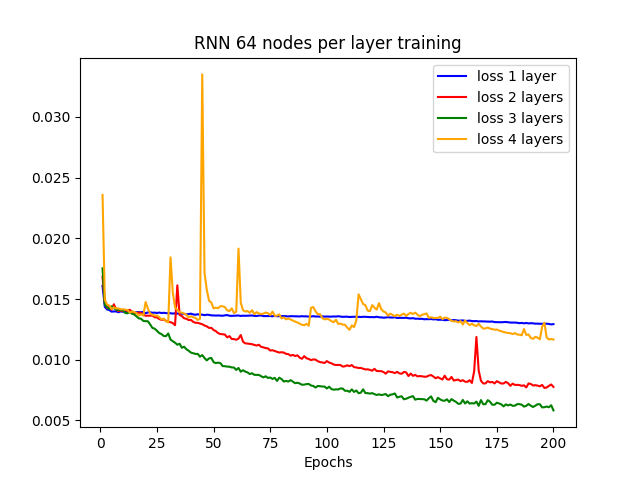
\includegraphics[width=\linewidth]{../TESTS_RESULTS/RNN_tests/plots/64_training.png} 
	\end{minipage}%%
	\begin{minipage}[b]{0.33\linewidth}
		\centering
		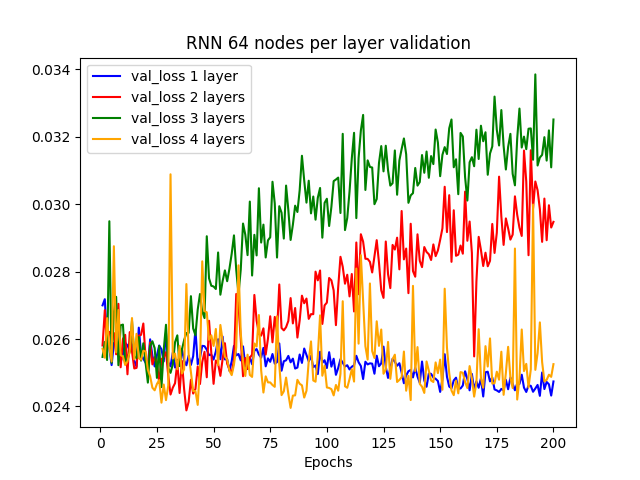
\includegraphics[width=\linewidth]{../TESTS_RESULTS/RNN_tests/plots/64_validation.png} 
	\end{minipage} 
	\begin{minipage}[b]{0.33\linewidth}
		\centering
		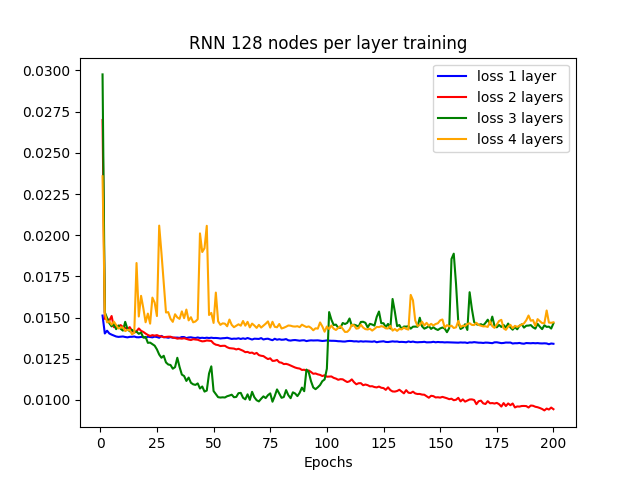
\includegraphics[width=\linewidth]{../TESTS_RESULTS/RNN_tests/plots/128_training.png} 
	\end{minipage}%% 
	\begin{minipage}[b]{0.33\linewidth}
		\centering
		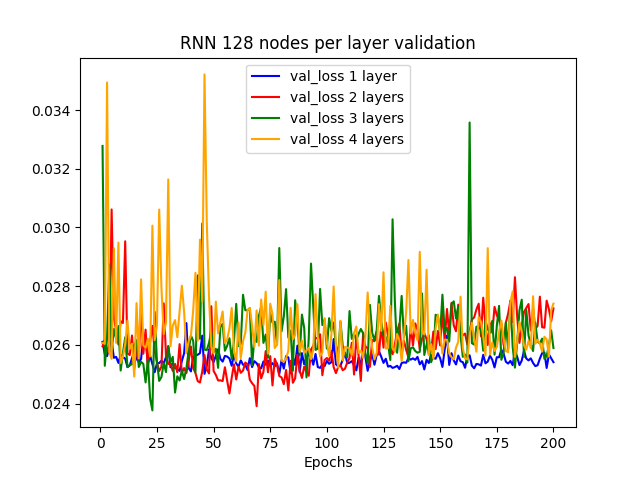
\includegraphics[width=\linewidth]{../TESTS_RESULTS/RNN_tests/plots/128_validation.png} 
	\end{minipage} 
\hspace*{-2cm}  
	\begin{minipage}[b]{0.33\linewidth}
		\centering
		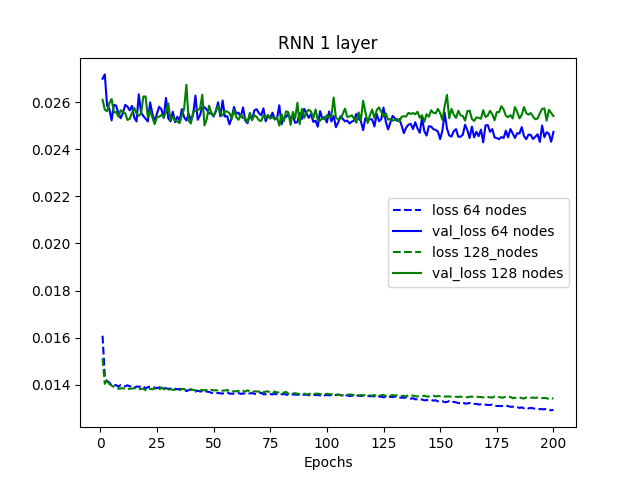
\includegraphics[width=\linewidth]{../TESTS_RESULTS/RNN_tests/plots/1_comp.png} 
	\end{minipage}%%
	\begin{minipage}[b]{0.33\linewidth}
		\centering
		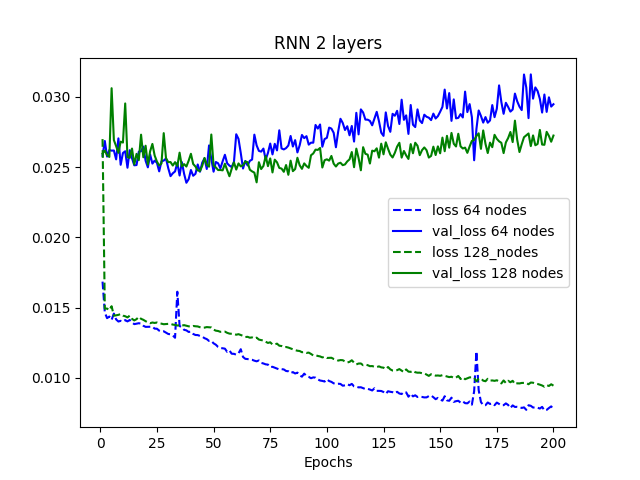
\includegraphics[width=\linewidth]{../TESTS_RESULTS/RNN_tests/plots/2_comp.png} 
	\end{minipage} 
	\begin{minipage}[b]{0.33\linewidth}
		\centering
		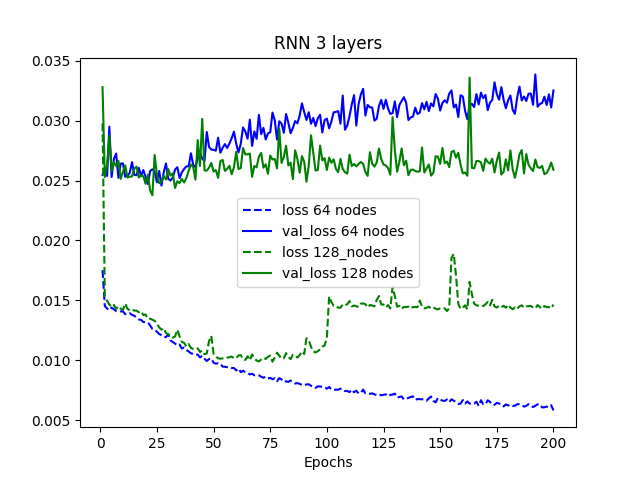
\includegraphics[width=\linewidth]{../TESTS_RESULTS/RNN_tests/plots/3_comp.png} 
	\end{minipage}%% 
	\begin{minipage}[b]{0.33\linewidth}
		\centering
		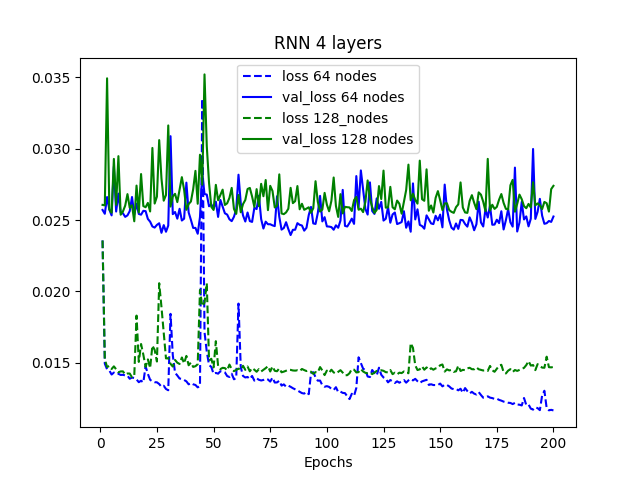
\includegraphics[width=\linewidth]{../TESTS_RESULTS/RNN_tests/plots/4_comp.png} 
	\end{minipage} 
	\caption{Results from RNN models} 
\label{fig:RNNplots}
\end{figure}


If we have a look at the resulting plots of \textbf{figure}~\ref{fig:RNNplots}, we see large fluctuation of the loss function when validating the models. The general trend of the loss for a 64 node per layer model is a drop around 0.025 between 25 and 50 epochs. The model with 3 hidden layers starts to gain the most lost the quickest and the simplest one with one layer continues to drop to a loss of around 0.024. The validation of the 128 nodes variant  fluxes the most and tends to average around 0.026 for any amount of layers.
\\
The RNN model with 3 layers shows the most divergent loss functions between the 64 and 128 nodes variant. For the 4 layer variants we can observe a huge spike in validation loss when training loss spikes. This does not immediately indicates a correlation between both functions rather it could be similar impactful, yet different entries that generated a big spike in both training an validation in the proximity of that epoch.


\subsection{LSTM}
\begin{figure}[H] 
	\hspace*{-2cm}  
	\begin{minipage}[b]{0.33\linewidth}
		\centering
		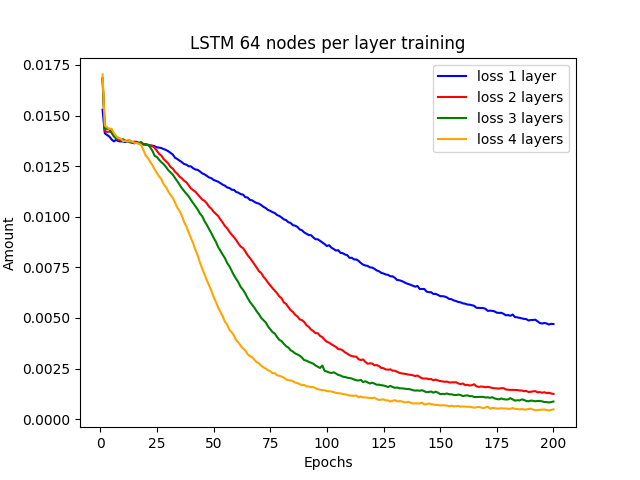
\includegraphics[width=\linewidth]{../TESTS_RESULTS/LSTM_tests/plots/64_training.png} 
	\end{minipage}%%
	\begin{minipage}[b]{0.33\linewidth}
		\centering
		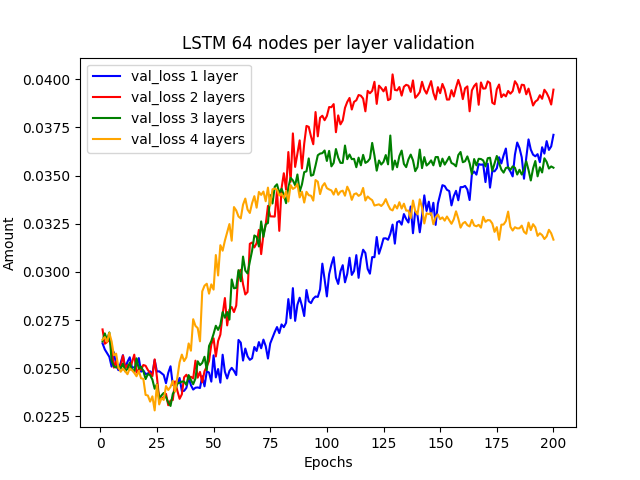
\includegraphics[width=\linewidth]{../TESTS_RESULTS/LSTM_tests/plots/64_validation.png} 
	\end{minipage} 
	\begin{minipage}[b]{0.33\linewidth}
		\centering
		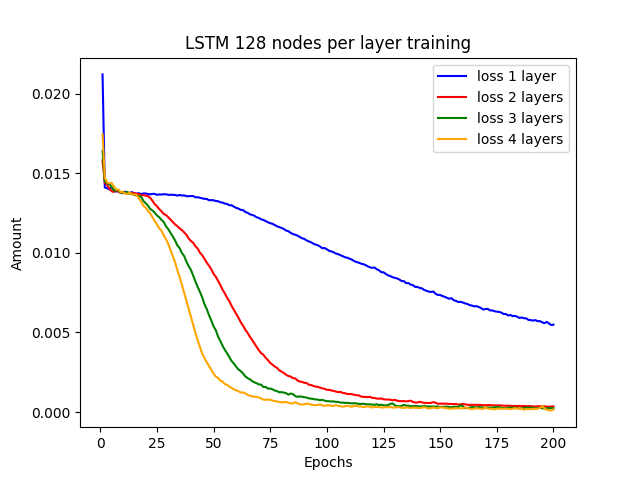
\includegraphics[width=\linewidth]{../TESTS_RESULTS/LSTM_tests/plots/128_training.png} 
	\end{minipage}%% 
	\begin{minipage}[b]{0.33\linewidth}
		\centering
		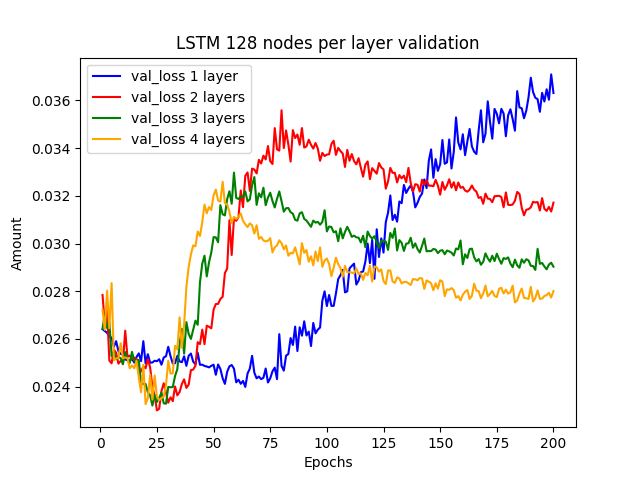
\includegraphics[width=\linewidth]{../TESTS_RESULTS/LSTM_tests/plots/128_validation.png} 
	\end{minipage} 
\hspace*{-2cm}  
	\begin{minipage}[b]{0.33\linewidth}
		\centering
		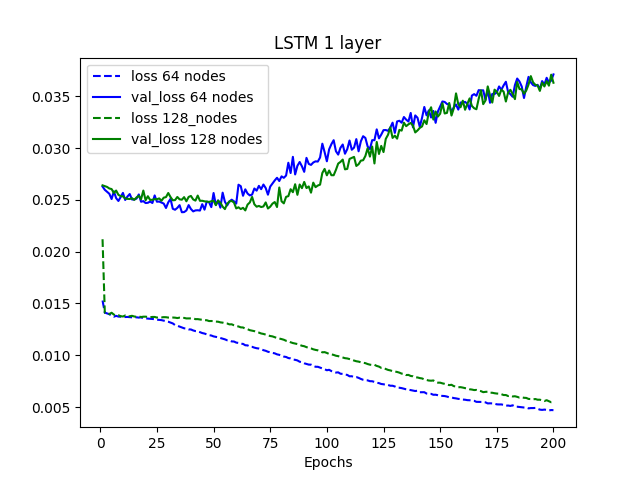
\includegraphics[width=\linewidth]{../TESTS_RESULTS/LSTM_tests/plots/1_comp.png} 
	\end{minipage}%%
	\begin{minipage}[b]{0.33\linewidth}
		\centering
		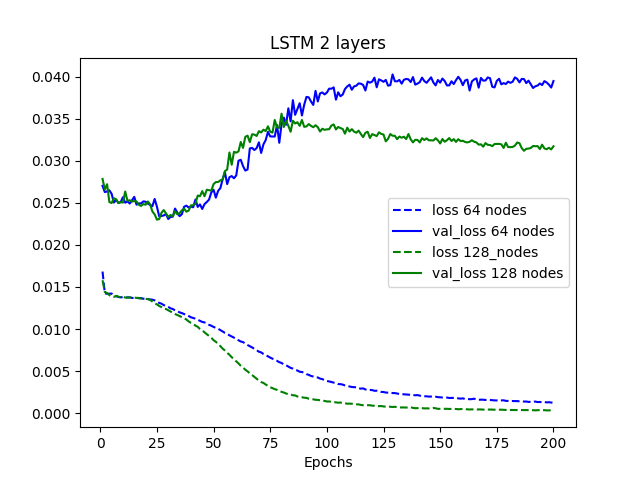
\includegraphics[width=\linewidth]{../TESTS_RESULTS/LSTM_tests/plots/2_comp.png} 
	\end{minipage} 
	\begin{minipage}[b]{0.33\linewidth}
		\centering
		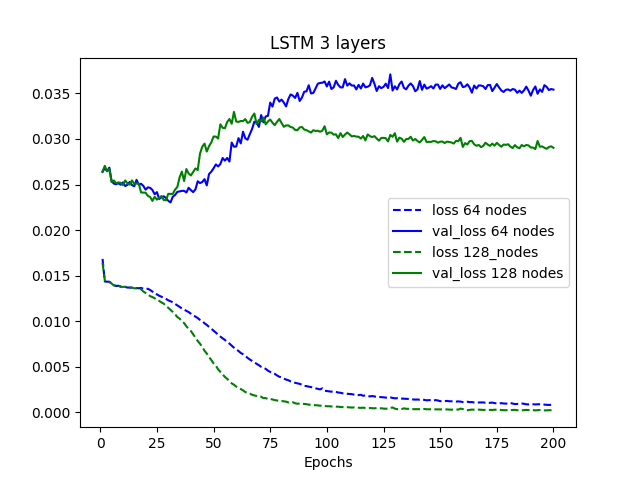
\includegraphics[width=\linewidth]{../TESTS_RESULTS/LSTM_tests/plots/3_comp.png} 
	\end{minipage}%% 
	\begin{minipage}[b]{0.33\linewidth}
		\centering
		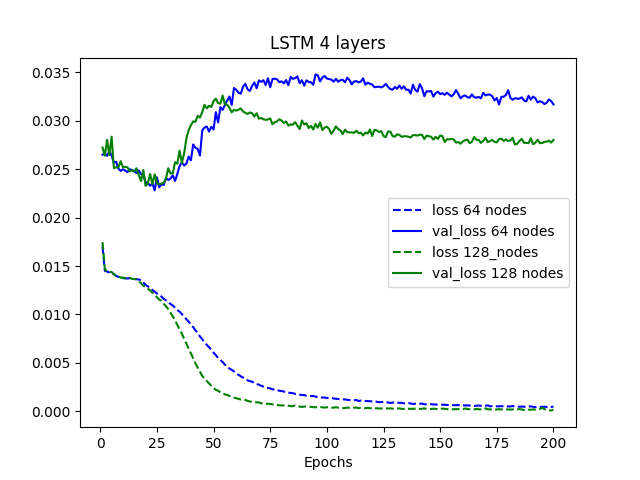
\includegraphics[width=\linewidth]{../TESTS_RESULTS/LSTM_tests/plots/4_comp.png} 
	\end{minipage} 
\caption{Results from LSTM models} 
\label{fig:LSTMplots}
\end{figure}

In \textbf{figure}~\ref{fig:LSTMplots} we can observe a similar trend for the loss functions of different models and in general less sporadic fluctuations then the RNN ones . The loss starts with a significant drop to a local minimum before gradually rising again. At different epochs we then observe a ceiling for the function and a consecutive decrease. This trend however is not noticeable for the simple 1 layered model as it keeps increasing in loss, even after the experiment's limit of  200 epochs.
\\
For a 64 nodes model, we can conclude overfitting will occur after the local minimum of the validation loss function at around +30 epochs for more then one layer models and around +45  epochs for the single layered one. For the 128 nodes variant we observe a significant increase in epochs needed for overfitting the 1 layer model compared to the other ones. While they have their loss minimum at 25 epochs, the single layer reach it at 75 epochs.
\\
As for the training part of the loss functions, we observe much smoother ones then those of the trained RNN models.

\subsection{GRU}
Last we run experiments with the GRU variant of RNN's. 

\begin{figure}[H] 
	\hspace*{-2cm}  
	\begin{minipage}[b]{0.33\linewidth}
		\centering
		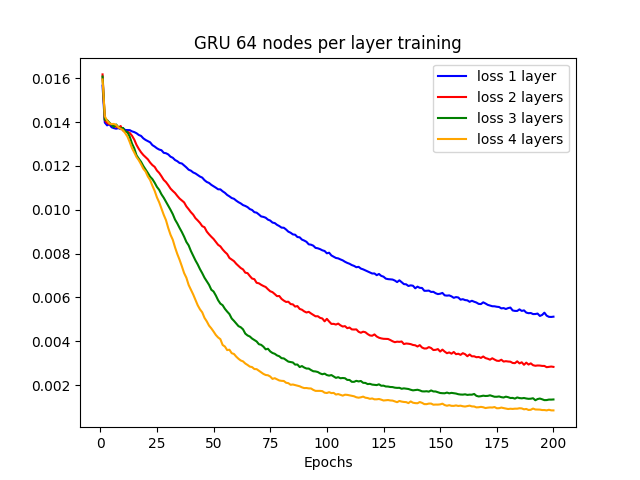
\includegraphics[width=\linewidth]{../TESTS_RESULTS/GRU_tests/plots/64_training.png} 
	\end{minipage}%%
	\begin{minipage}[b]{0.33\linewidth}
		\centering
		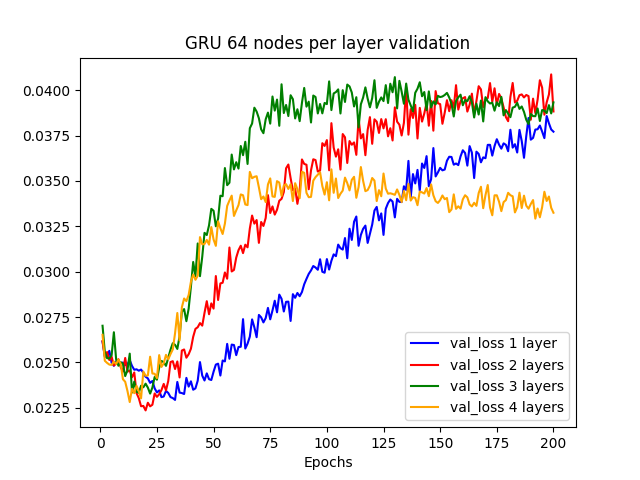
\includegraphics[width=\linewidth]{../TESTS_RESULTS/GRU_tests/plots/64_validation.png} 
	\end{minipage} 
	\begin{minipage}[b]{0.33\linewidth}
		\centering
		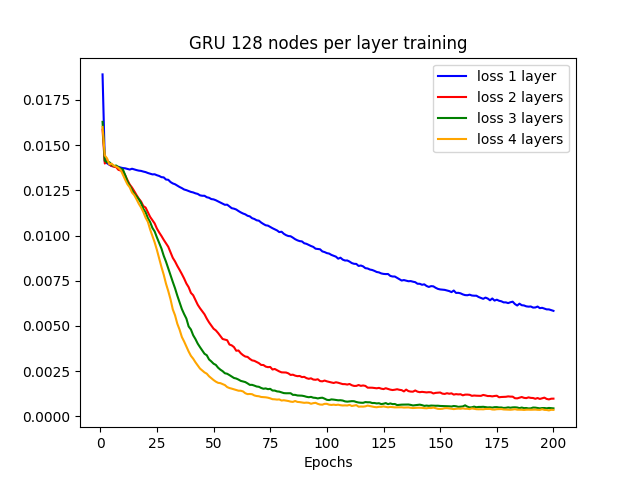
\includegraphics[width=\linewidth]{../TESTS_RESULTS/GRU_tests/plots/128_training.png} 
	\end{minipage}%% 
	\begin{minipage}[b]{0.33\linewidth}
		\centering
		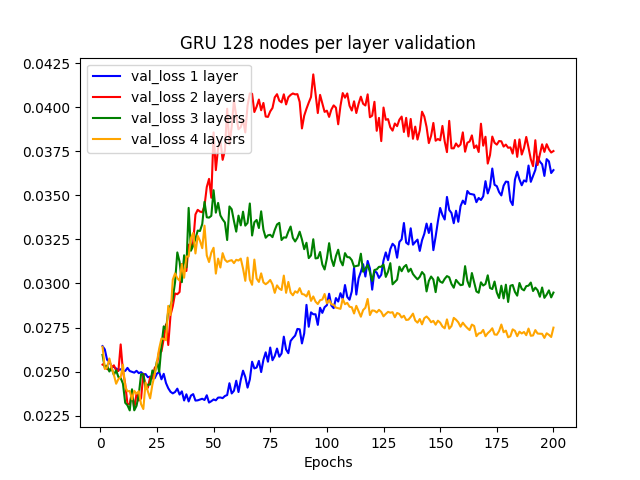
\includegraphics[width=\linewidth]{../TESTS_RESULTS/GRU_tests/plots/128_validation.png} 
	\end{minipage} 
	\hspace*{-2cm}  
	\begin{minipage}[b]{0.33\linewidth}
		\centering
		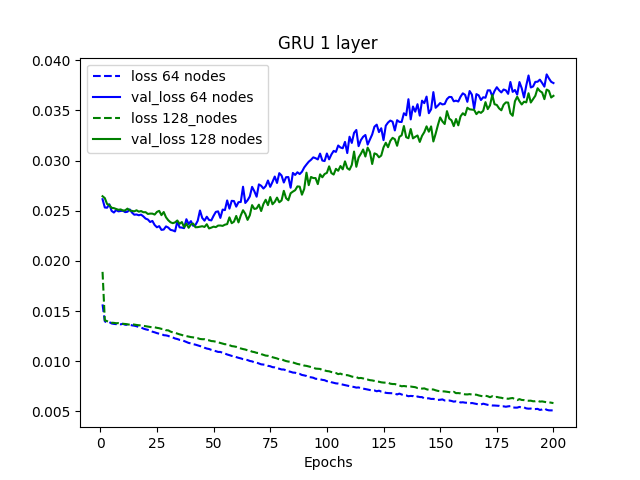
\includegraphics[width=\linewidth]{../TESTS_RESULTS/GRU_tests/plots/1_comp.png} 
	\end{minipage}%%
	\begin{minipage}[b]{0.33\linewidth}
		\centering
		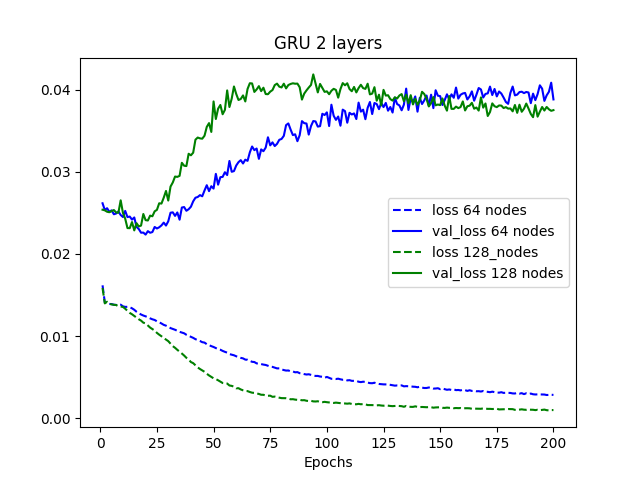
\includegraphics[width=\linewidth]{../TESTS_RESULTS/GRU_tests/plots/2_comp.png} 
	\end{minipage} 
	\begin{minipage}[b]{0.33\linewidth}
		\centering
		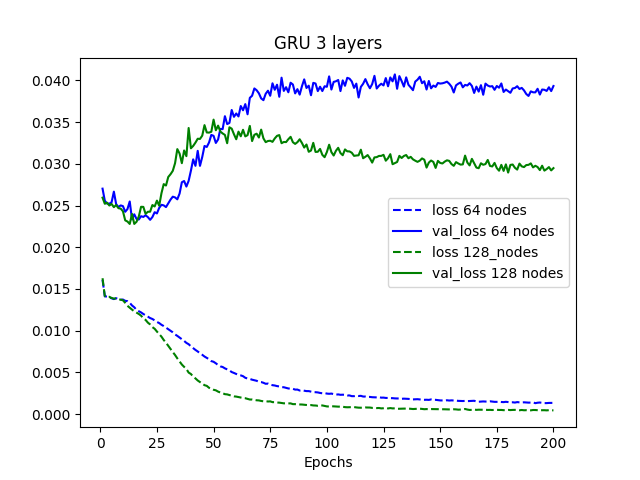
\includegraphics[width=\linewidth]{../TESTS_RESULTS/GRU_tests/plots/3_comp.png} 
	\end{minipage}%% 
	\begin{minipage}[b]{0.33\linewidth}
		\centering
		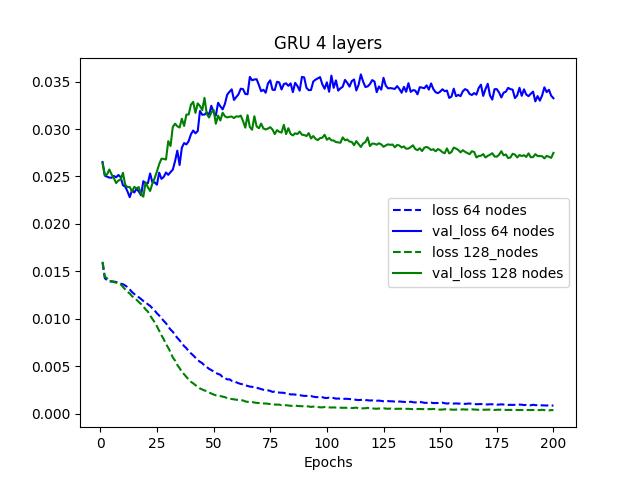
\includegraphics[width=\linewidth]{../TESTS_RESULTS/GRU_tests/plots/4_comp.png} 
	\end{minipage} 
	\caption{Results from GRU models} 
	\label{fig:GRUplots}
\end{figure}

For the trained GRU models (\textit{figure 4}) we can observe similar trends as in the LSTM models. GRU models tend to reach a local minimum in their validation loss function around 5 epochs earlier then the LSTM models. 
\\
We can observe a higher maximum in the validation loss of the 3 layer models compared to the equivalent LSTM models for both 64 And 128 nodes. For the 2 layer models, we see a higher increase in validation loss for the more complex 128 nodes variant then the LSTM for small number of epochs (< 100) . However, the validation loss of the less complex 2 layer model catches up around 150 epochs and achieves the highest maximum of both models at 200 epochs.


\section{Evaluation}

\subsection{With plots of the loss function}
We cannot evaluate the quality of the music generated with those plots.
In one hand we cannot really validate the training data with a validation data, since the validation data are two different compositions and it is \textit{impossible} that the network predicts the sequences of a new song base solely.
It is normal that the the validation and training loss error grow apart in the plots.
But in the other hand, since we are training with a particular theme: Chopin's Nocturnes, we do not want them to grow too much apart, we want to generalize the theme and the network learns the \textit{style} of Chopin's Nocturnes.\\
So in for one part we cannot avoid overfitting, and even we want it to overfit, but we do not want that this overfitting is too important in order to generate \textit{new} music.
\\

With the exception of Vanilla RNN, the validation loss error tends to grow and then reach a point were it \textit{stabilizes} or even in some cases it decreases.\\
Those parts could be explained as when the model learns the training music a little, therefore the validation music differs from the training model and the error grows.
And when the validation loss error starts to decrease we could think that the network learned better the sequences of notes that go good together so the error in validation decreases.\\
The GRU model with 4 layers and 128 hidden units is a good example of this \textbf{figure}~\ref{fig:GRUplots}.\\
\\
For the Vanilla RNN just watching the plots of the loss function, one could say that the network barely learns something with models with 64 hidden units per layer, and not at all with the models with 128 hidden units per layer.\\
But what does the music produced sounds like?


\subsection{Comparing the music}

The best way to evaluate the results is evaluating the music generated by the model. But even there it is a subjective matter. \\
The first thing that we can describe is that the the first few seconds of the song is a bunch of chords and notes pressed almost simultaneously.
Then a sequence of notes more melodic/harmonic that sounds more as music proceeds.
It ends with a repetitive pattern of sparse notes from here and there.
This is the general structure for all the music produced by our models.
Let's take into account that the way we encode again the results into midi files again might have some effects on this too.\\
We are going too compare the \textit{harmonic} part of the music for each model.\\
\\

Comparing the music generated by the most simple models, (GRU, LSTM, RNN, with 64 hidden units and 1 layer) we were not surprised by the results after analyzing the plots.
The RNN model sounded like a child fiddling kindly with a piano repeating some patterns.
The LSTM model sounded like a non musician adult playing around with a piano trying new sounds that might be pleasant.
The GRU model sounded like a musician of contemporary music exploring random sounds.\\
The best model in our opinion was the the GRU one and the worst was the RNN.
They all sound weird and might made no sense, but in some way the GRU model was more pleasant to our ears and sounded like made a little bit more sense than the others.\\
\\

Now, comparing the most complex model with the simplest model of GRU architectures (GRU with 1 layer and 64 hidden units against GRU with 4 layers and 128 hidden units), they are both really similar at some points we can think hearing Chopin even though within the big picture it's still really messy as music. 
But the most complex model is a little bit more musical, with more harmonics, and we kind of see some evolution in the music, like a song that tells a story, meanwhile the simplest model is less melodic and more continuous.\\
\\
As an interesting note, people who have heard the music tend to add to their description some components that describe Chopin's Nocturnes, like \textit{classical and dark.}
One interesting thing would have the opinion of an expert to see if some harmonic patterns are learned.\\


\section{Conclusion}
RNNs can generate music. 
Given a good training set the network could learn sequence of notes that are good to hear and maybe avoid sequences that do not sound good.
But how \textit{creative} could it get?\\
One of the main difficulties with this approach is that evaluating music is really subjective.
There is not a metric that can objectively evaluate how good a sequence of notes is.\\
One of our main problems that we can see is how bad the accuracy was when comparing the training set with a validation set.
This is not surprising, since,  even though the compositor was the same and the style was similar (we only worked on the Chopin's Nocturnes), the songs in the validation set were different and new from the training set.\\
\\

The music generated is weird and messy, it is clear it was not  a musician who wrote it. But we detected some hints of Chopin's Nocturne essence.
The LSTM and GRU models kind of learn something, and each different architecture produces different musics.\\
\\

For further work on this we could see the effect of changing the \textit{windowing} for the sequence of notes in the training set.
And to produce more realistic music add the tempo to the pitch to produce real notes.\\
Also add more epochs to see if the model can learn better and yield better results could be another interesting experiment.\\
We do believe that some interesting music can be generated with RNNs but never as good and creative as humans.

\bibliographystyle{apacite}
\bibliography{references}

\end{document}